\begin{textblock}{21}[0,0](0,0.2)
    \ifnum \APforPrint=0
        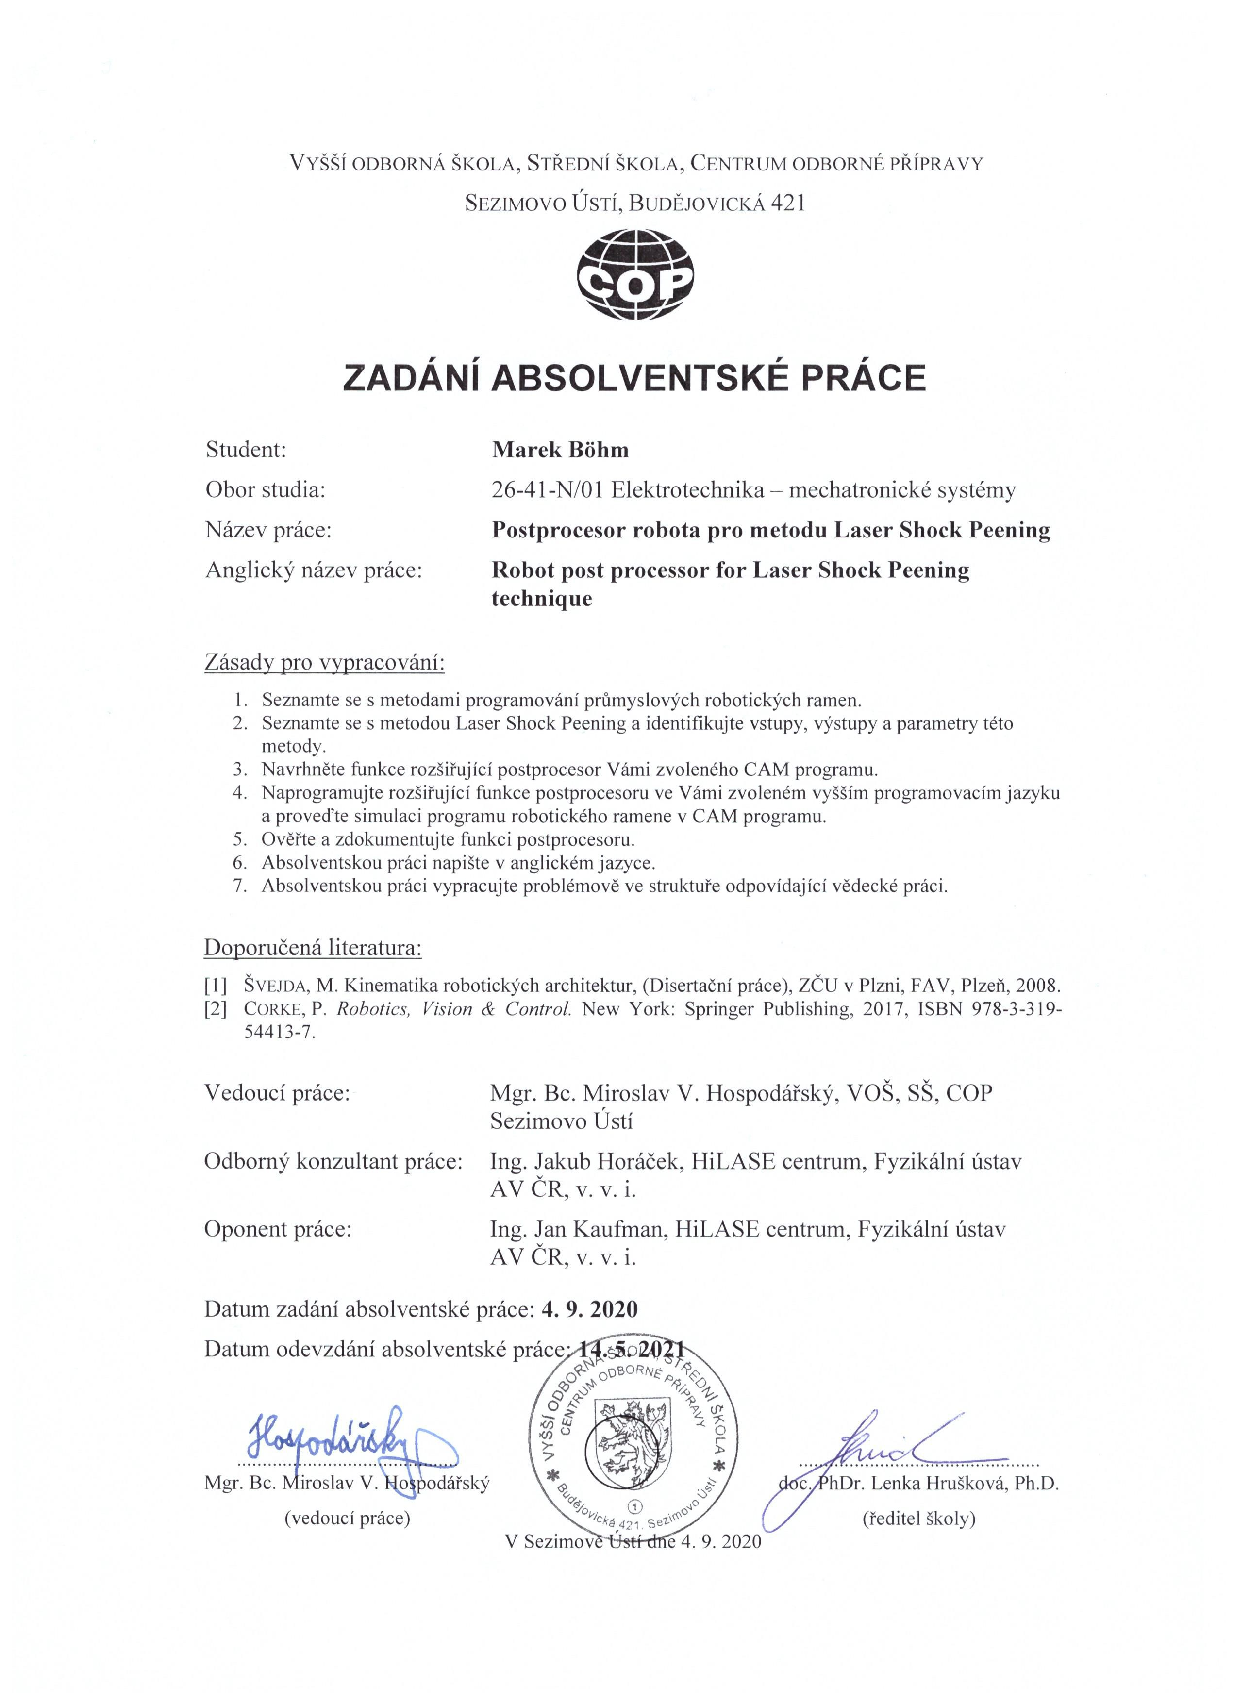
\includegraphics[width=21cm]{\cestaFiles Figures/Scan/assignment_scan.pdf}
    \else
        \vglue 13cm
        \hspace{5cm}
        {\huge Zde vložte originál zadání!!!}
    \fi
\end{textblock}

%%% Odtud mazat "barevný" text
\textcolor{red}{\em Místo tohoto listu vložte do tištěné práce originální zadání Vaší práce (podepsané vedoucím a~ře\-di\-te\-lem)!!!\/}

\textcolor{blue}{\em Také do finálního PDF souboru s~Vaší AP, kterou vypálíte na CD/DVD a~nahrajete na MOODLE, vložte naskenované vedoucím a ředitelem podepsané originální zadání.\/}

\textcolor{blue}{\em Můžete postupovat takto. Naskenujte celou A4 originálního podepsaného zadání do souboru \texttt{task.jpg} (rozlišení cca 1700$\times$2404). Tento naskenovaný jpg-soubor uložte do složky \texttt{00\_files/Figures/Scan/}. Nakonec překonvertujte \texttt{task.jpg} na \texttt{task.eps}. Ke konverzi do formátu EPS možno využít matlabovský m-file \texttt{ScanAPjpg2eps.m}, který stačí spustit.\/}

\textcolor{blue}{\em Tento text se nachází na konci souboru \texttt{00\_files/Task.tex}. V~momentě, kdy výše uvedené provedete, tento barevný text vymažte.\/} 
%%% sem mazat "barevný" text 
